%%%%%%%%%%%%%%%%%%%%%%%%%%%%%%%%%%%%%%%%%%%%%%%%%%%%%%%%%%%%%%%%%%%%%%%%
\chapter{Evaluation} \label{Evaluation}
%%%%%%%%%%%%%%%%%%%%%%%%%%%%%%%%%%%%%%%%%%%%%%%%%%%%%%%%%%%%%%%%%%%%%%%%
We conduct several experiments to understand the latency and throughput of our system under various conditions. Our key takeaways are as follows:

\begin{enumerate}
    \item Our approach using asynchronous, lock-free cache updates can improve end-to-end inference latency up to 28\%. Our frequency-based admission and eviction policy can outperform LFU in terms of cache hit rate, and our asynchronous update mechanism can avoid additional overheads.
    \item By splitting a logical cache among GPUs connected by NVLink, our system's throughput can scale linearly. 
    \item Our lock-free approach improves P99 latency over naive locking using a reader-write lock. While we don't see a noticable improvement in peak throughput when using locking vs. lock-free, a microbenchmark in Section \ref{Eval: microbenchmark} highlights how lock contention worsens as the number of GPUs in the system increase.
\end{enumerate}

%%%%%%%%%%%%%%%%%%%%%%%%%%%%%%%%%%%%%%%%%%%%%%%%%%%%%%%%%%%%%%%%%%%%%%%%
\section{Experimental Setup}
%%%%%%%%%%%%%%%%%%%%%%%%%%%%%%%%%%%%%%%%%%%%%%%%%%%%%%%%%%%%%%%%%%%%%%%%
\subsection{Environment} \label{Eval: Test hardware}
We primarily test on one machine, equipped with two 16-core Intel Xeon Silver 4314 CPUs \@ 2.4 GHz, 256 GB main memory, and two NVIDIA 80 GB A100 GPUs connected with NVLinks. We run on Ubuntu 20.04 with kernel version 5.15.0-25-generic, PyTorch 13.1, DGL 1.0, and CUDA 11.7.

\subsection{Datasets \& Workloads}
We evaluate our system using four graph datasets, summarized in Table \ref{Eval: Dataset info}.
\begin{table}[h!]
    \begin{center}
        \begin{tabular}{|c c c c c|} 
        \hline
        \textbf{Dataset} & \textbf{Nodes} & \textbf{Edges} & \textbf{Features} & \textbf{Avg. Degree} \\ [0.5ex] 
        \hline\hline
        reddit \cite{GraphSAGE_2017} & 200K & 111M & 602 & 492 \\
        \hline
        yelp \cite{GraphSAINT_2019} & 700K & 13M & 500 & 10 \\
        \hline
        ogbn-products \cite{OGB_2020} & 2.4M & 124M & 100 & 51.7 \\
        \hline
        ogbn-papers100M \cite{OGB_2020} & 111M & 1.6B & 128 & 14.4 \\
        \hline
        \end{tabular}
    \end{center}
    % ogbn-products, uniform sampling, batch size 256, total latency 
    \caption{Graph datasets used in evaluation}
    \label{Eval: Dataset info}
\end{table}
Since we could not find any publicly available GNN inference traces, we create our own by removing 10\% of nodes from each graph to serve as inference target nodes. We create requests from these nodes by using their original features and edges. 

To emulate different types of inference traces, we create two varieties. 
\begin{description}
    \item[Uniform sampled requests] are generated by uniformly randomly sampling nodes from our pool of inference target nodes. These traces share similarity with mini-batch training and correspond to a somewhat worst case for dynamic caches, since there is little locality.
    \item[Subgraph biased requests] are generated by first partitioning the graph into $k$ partitions, and then cycling through each of the $k$ partitions, making them "hot". For the current "hot" partition, requests are drawn from that partition with a certain probability $x$. In our experiments we choose $k=5$ and $x=0.8$, although these parameters do not need to be fixed. We use DGL's built-in METIS \cite{METIS_1998} implementation for graph partitioning.
\end{description}
Since our optimizations are orthogonal to model performance, we conduct experiments primarily using a 2-layer GCN architecture. Our system generates full 2-hop neighborhoods when serving requests.

\subsection{Policies Evaluated}
Throughout our evaluation we compare several combinations of cache policies and mechanisms, summarized in Table \ref{Eval: Policy names}. The most important ones are in the first four rows. The Frequency Lock-free approach is our approach as described in Section \ref{Design}, with cache updates happening in a separate host thread and using the masked update mechanism for lock-free updates.
\begin{table}[h!]
    \begin{center}
        \begin{tabularx}{\textwidth}{|c X c X X|} 
        \hline
        \textbf{Policy name} & \textbf{Overview} & \textbf{Dynamic?} & \textbf{Cache replacement strategy} & \textbf{Sync. Mechanism}\\ [0.5ex] 
        \hline\hline
        Static & PaGraph static, degree-based cache & No & N/A & N/A \\
        \hline
        Frequency Prefetch & Prefetching strawman \ref{Design: strawman} & Yes & Replace cache every $k$ requests & R/W Lock \\
        \hline
        LFU & LFU & Yes & Evict least frequent in cache & R/W Lock \\
        \hline
        Frequency Lock-free $\star$ & Asynchronous, lock-free updates & Yes & Replace entries via \textit{cache candidates} & Lock-free \ref{Design: Lock-free} \\
        \hline
        Frequency R/W Lock & Asynchronous updates with R/W Lock & Yes & Replace entries via \textit{cache candidates} & R/W Lock \\
        \hline
        Frequency Synchronous & Synchronous updates & Yes & Replace entries via \textit{cache candidates} & R/W Lock \\
        \hline
        \end{tabularx} \\
        $\star$ is our approach
    \end{center}
    % ogbn-products, uniform sampling, batch size 256, total latency 
    \caption{Policy/mechanism combinations evaluated}
    \label{Eval: Policy names}
\end{table}
We do not include a no cache baseline since the static cache approach already produces 2-3x speedups in inference latency.

%%%%%%%%%%%%%%%%%%%%%%%%%%%%%%%%%%%%%%%%%%%%%%%%%%%%%%%%%%%%%%%%%%%%%%%%
\section{End-to-End Latency}
%%%%%%%%%%%%%%%%%%%%%%%%%%%%%%%%%%%%%%%%%%%%%%%%%%%%%%%%%%%%%%%%%%%%%%%%
We first compare examine request-response latency in a basic case where there is only one GPU and one InferenceEngine. This establishes the best case latency.
\begin{figure}[h!]
    \begin{minipage}[c]{0.499\textwidth}
        \centering
        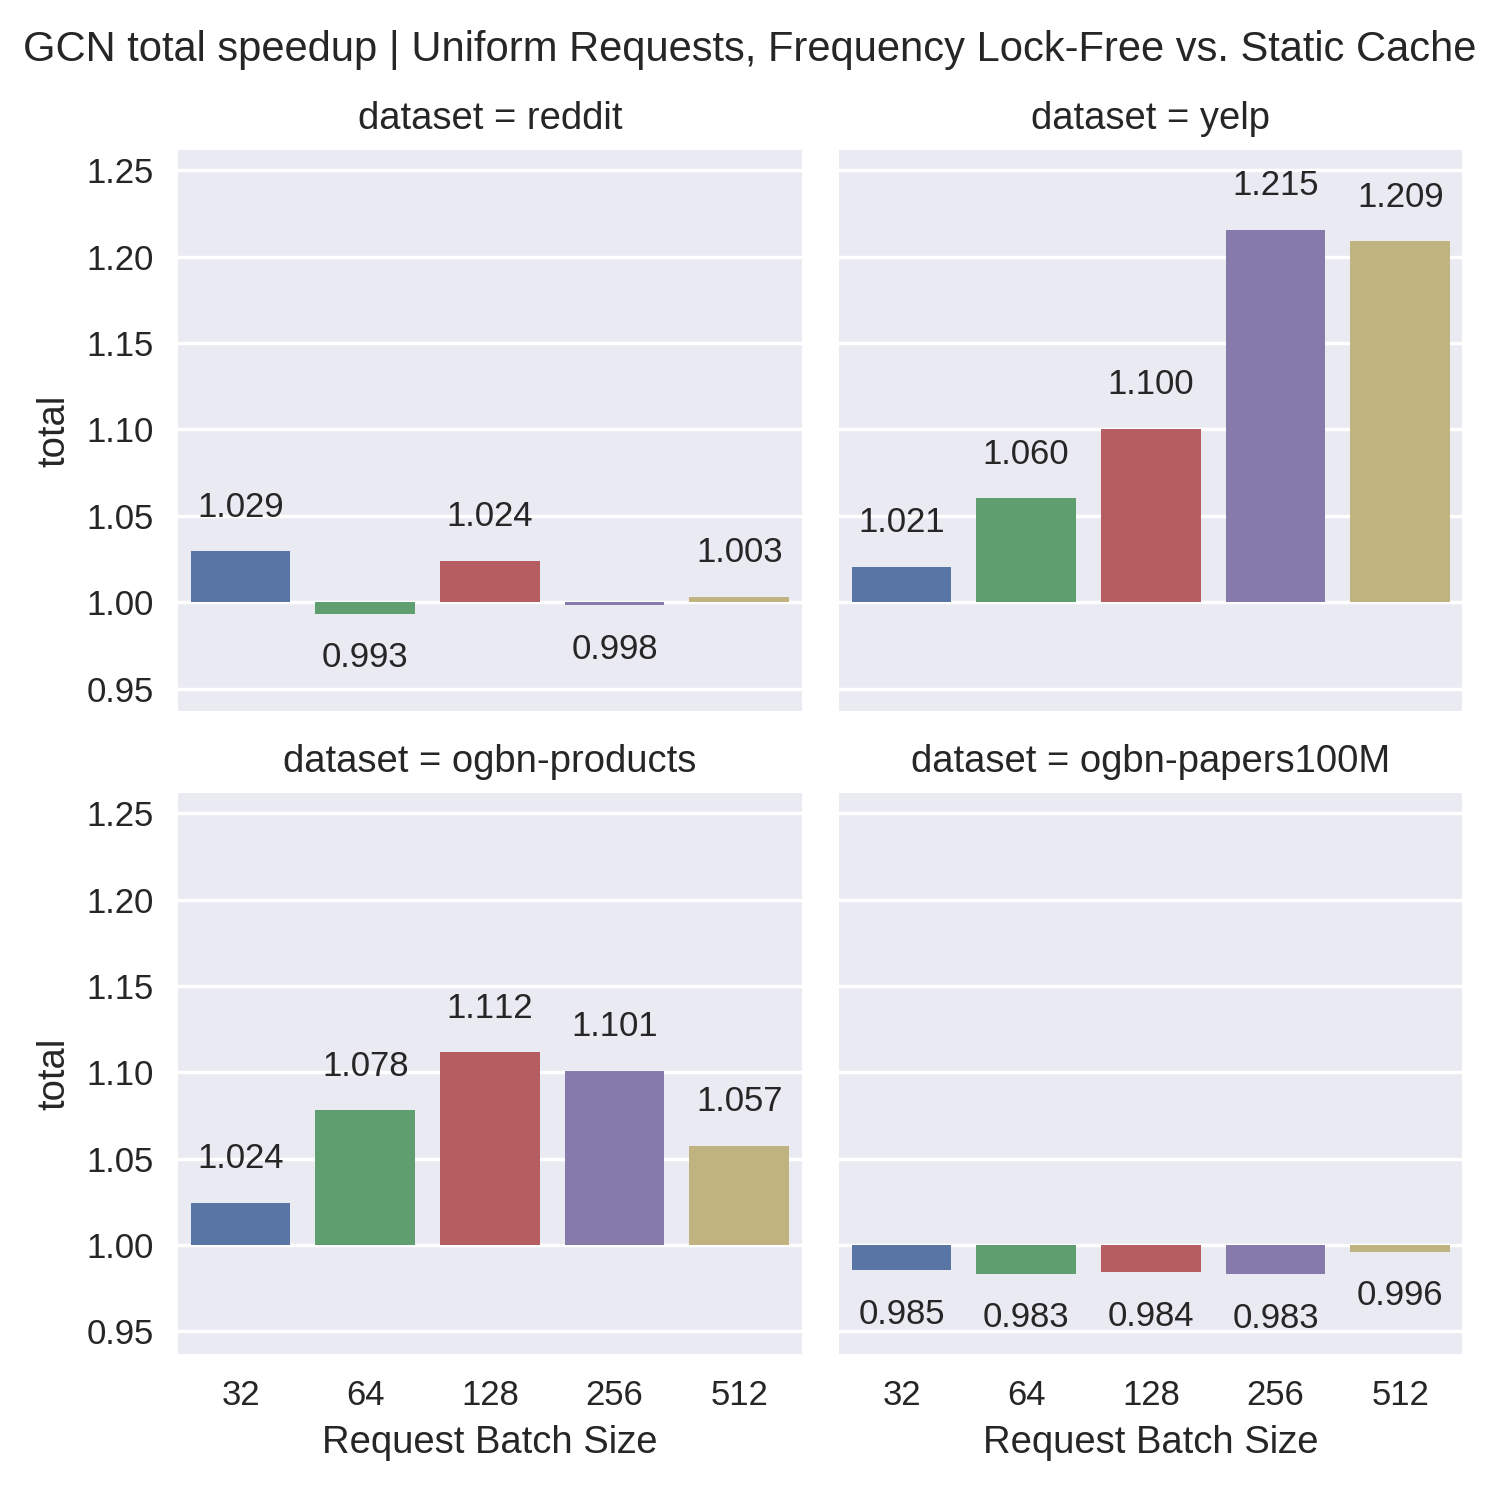
\includegraphics[width=\textwidth]{figures/speedup_GCN_total_uniform.png}
        \caption*{Uniformly sampled requests}
        % \caption{2-hop neighborhood and computation graph for node $A$, ignoring self loops.}
    \end{minipage}
    \hfill
    \begin{minipage}[c]{0.499\textwidth}
        \centering
        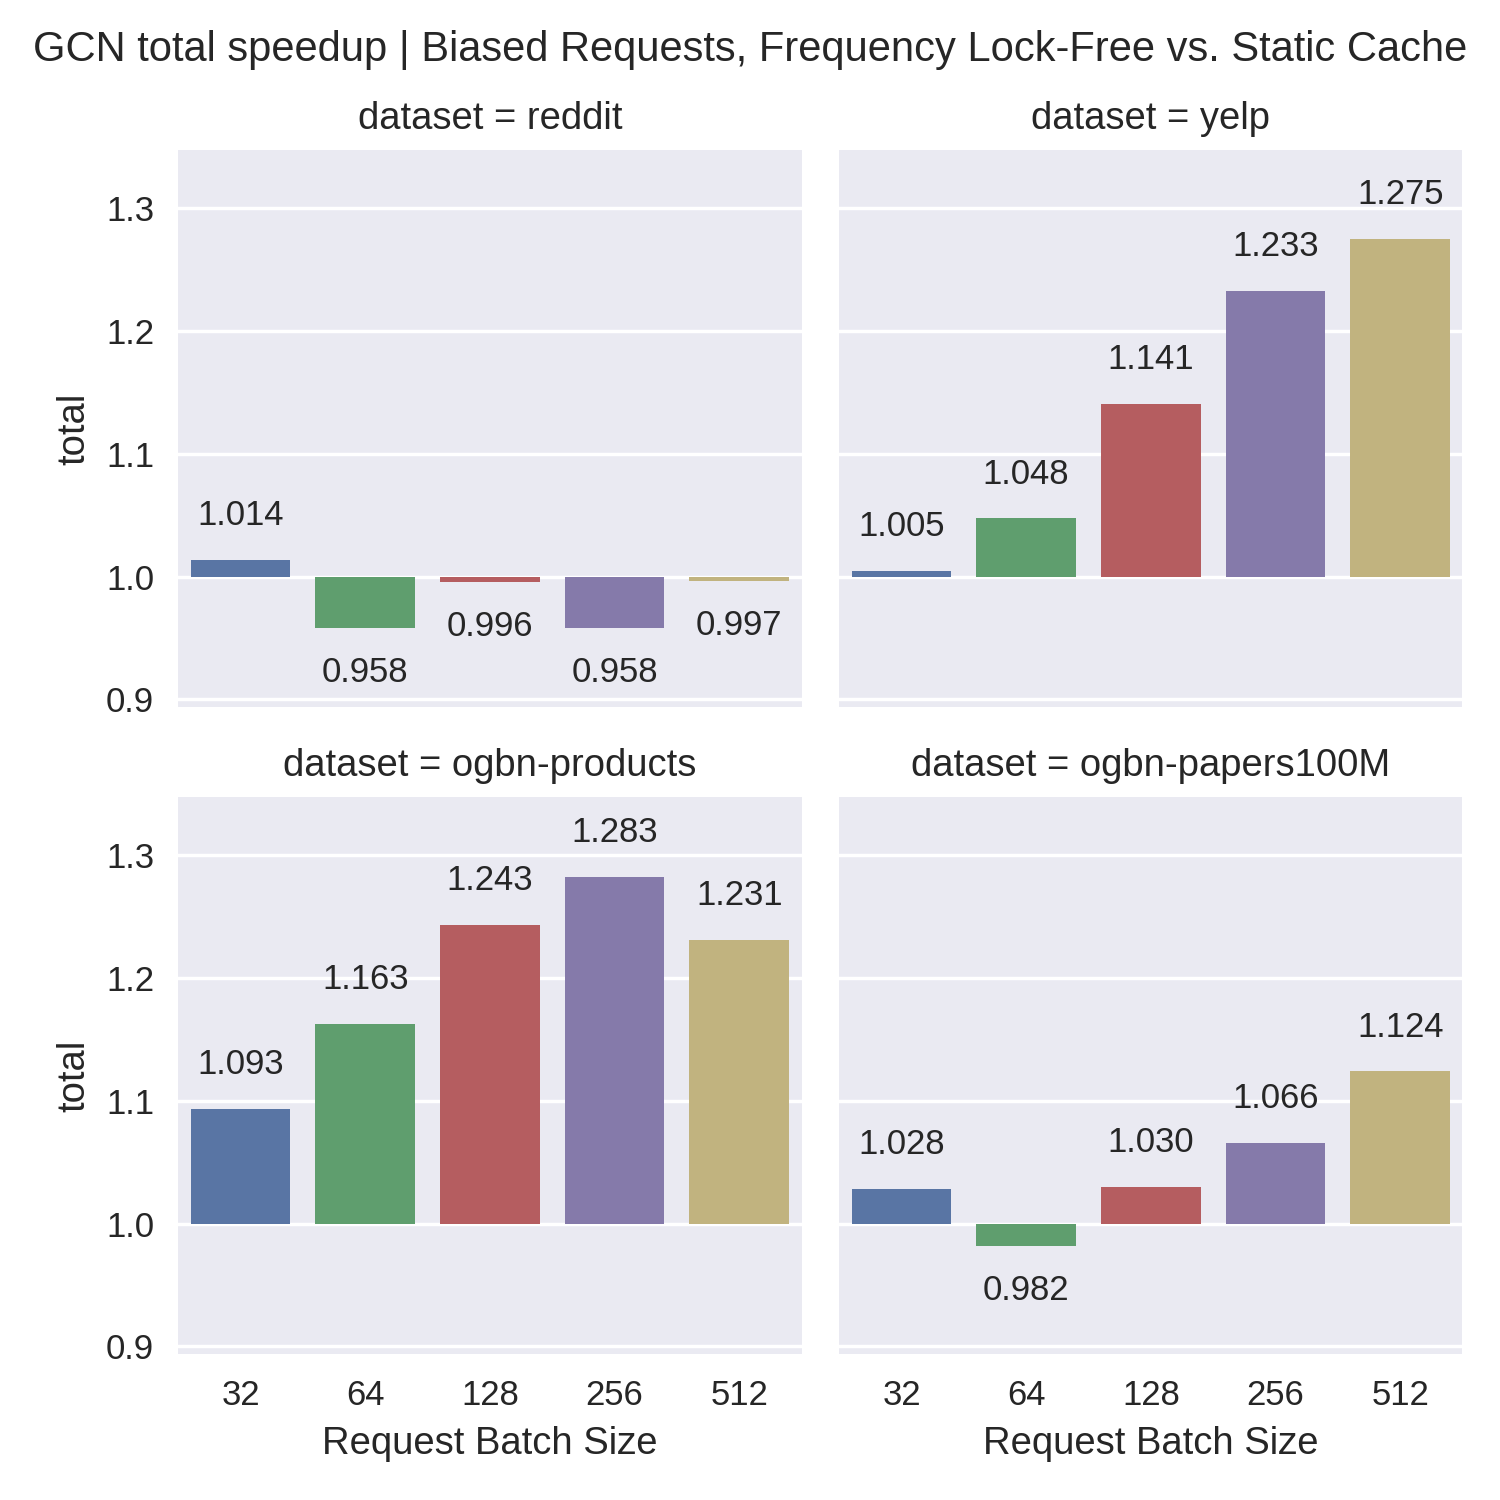
\includegraphics[width=\textwidth]{figures/speedup_GCN_total_bias.png}    
        \caption*{Subgraph biased requests}
        % \caption{Graph structure and associated node features (colored bars).}
    \end{minipage}
    \caption{End-to-end latency speedups for our lock-free asynchronous approach versus a static cache. Cache sizes are set to 20\% of total graph feature size.}
    \label{Eval: Speedups}
\end{figure}    
Figure \ref{Eval: Speedups} compares the speedup of our approach versus a static cache for both uniform and subgraph biased requests. For the yelp and ogbn-products datasets, our approach has speedups ranging from $0-28\%$. Interestingly, since the reddit dataset is incredibly dense, the frequency-based cache update heuristic is not able to achieve better cache hit rates, and this we do not see any speedup in either case. 

The ogbn-papers100M dataset is challenging because of its scale and sparsity, along with small feature dimension. Furthermore, the data loading phase was not that large of a proportion of end-to-end latency in the first place, as shown in Figure \ref{GPU Sampling Latency Breakdown}. In this case, increasing the request batch size helps improve inference latency with the dynamic cache since the frequency signal is stronger.

To understand these results better, in Figure \ref{Eval: Latency CDF} we also examine the CDFs of the same experiment but for all of the policies in Table \ref{Eval: Policy names} on ogbn-products batch size 256. Figure \ref{Eval: Hit Rate} shows the cache hit rates over time for the same experiments. We omit the Frequency Synchronous policy in the hit rate figures since it is the same as Frequency Lock-Free.

\begin{figure}[h!]
    \centering
    \begin{minipage}[c]{0.48\textwidth}
        \centering
        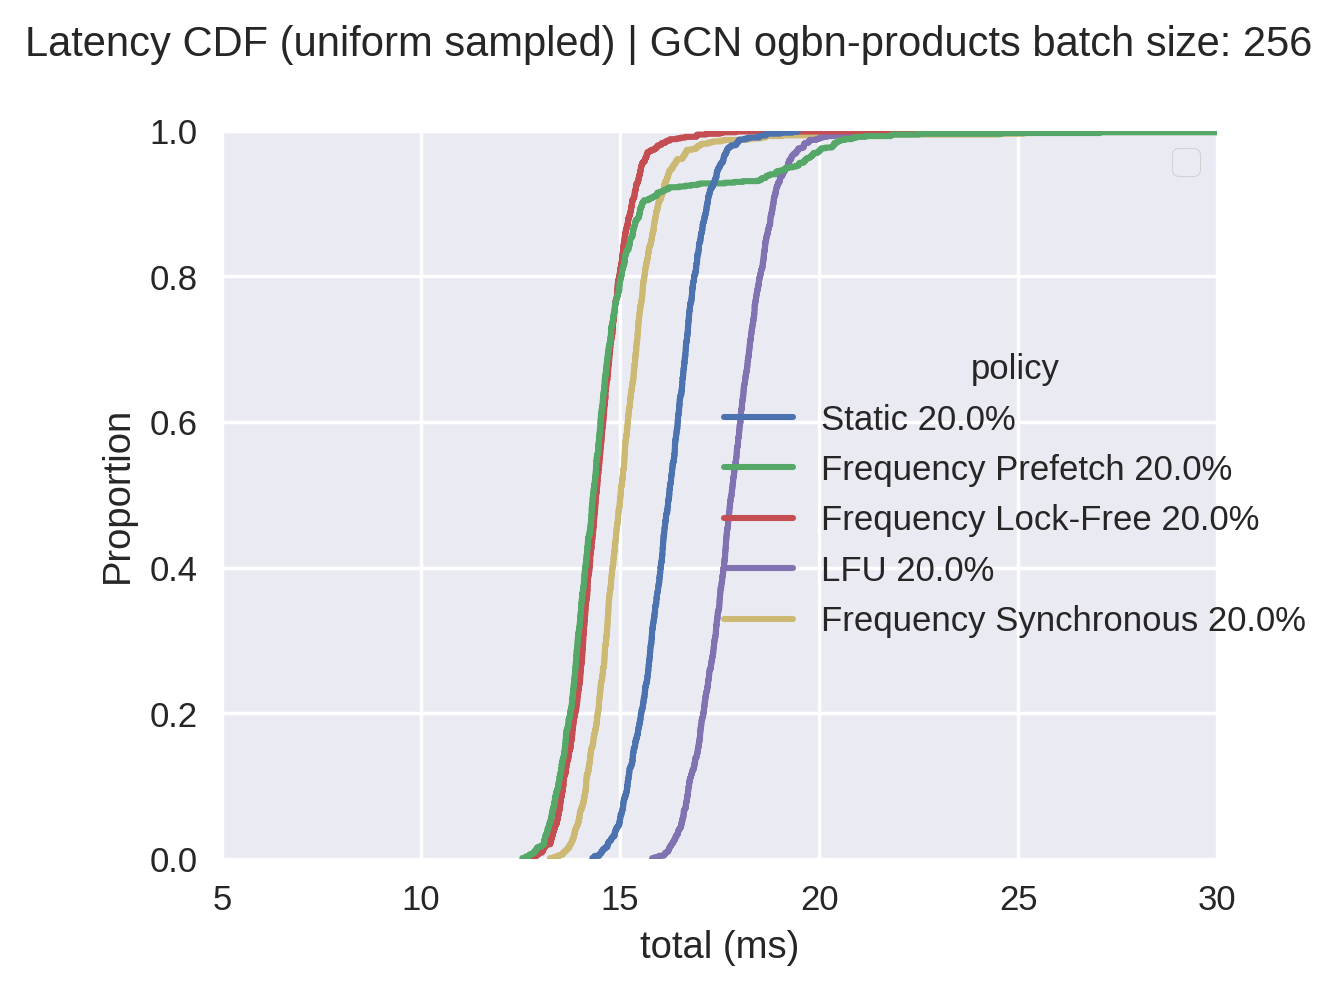
\includegraphics[width=\textwidth]{figures/CDF_GCN_uniform_pinnedc0.2.png}
        \caption*{Uniformly sampled requests}
    \end{minipage}
    \hfill
    \begin{minipage}[c]{0.48\textwidth}
        \centering
        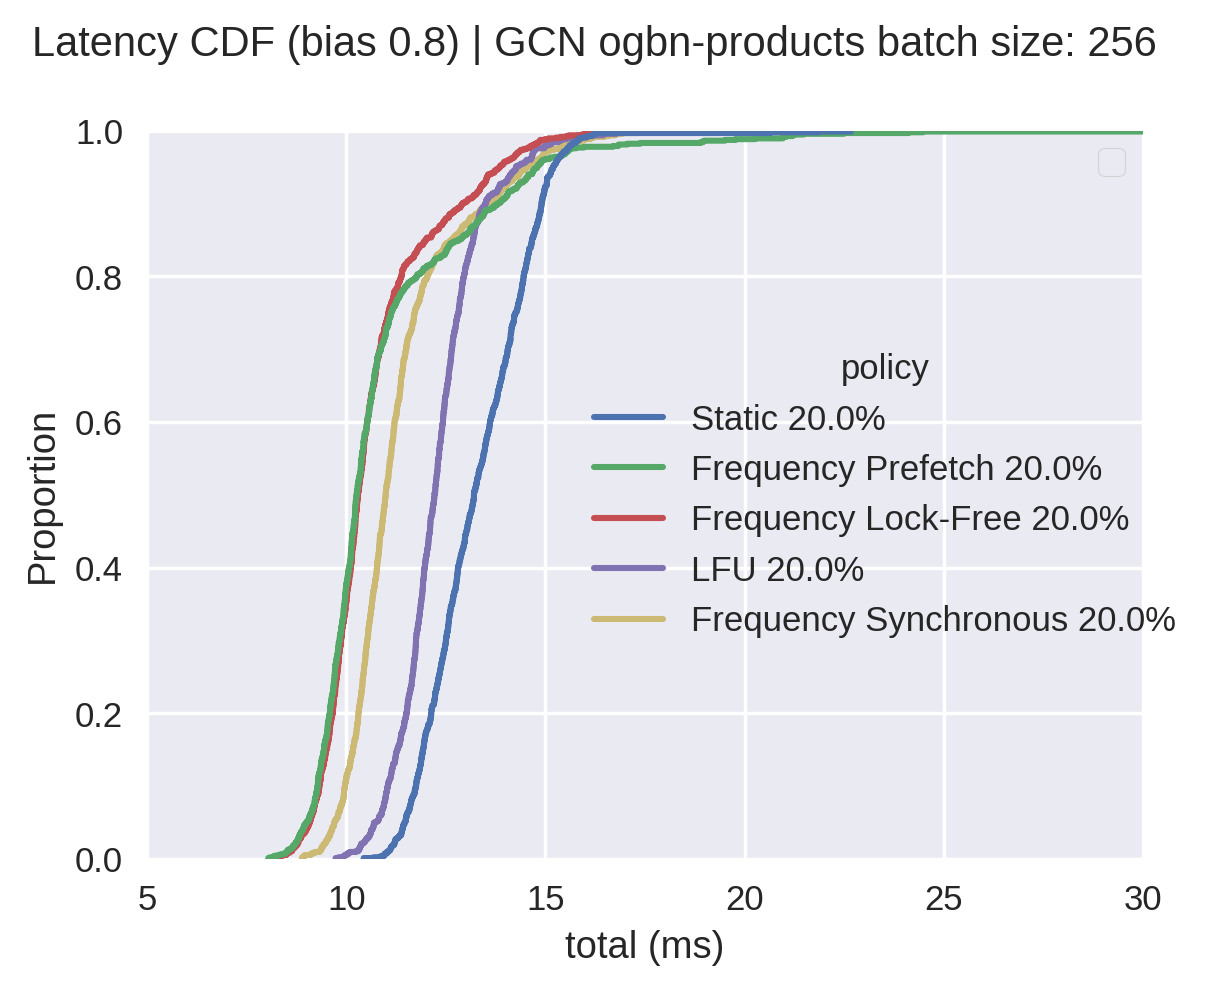
\includegraphics[width=\textwidth]{figures/CDF_GCN_bias_pinnedc0.2.png}    
        \caption*{Subgraph biased requests}
    \end{minipage}
    \caption{Latency CDFs for ogbn-products batch size 256}
    \label{Eval: Latency CDF}
\end{figure}    

\begin{figure}[h!]
    \centering
    \begin{minipage}[c]{0.48\textwidth}
        \centering
        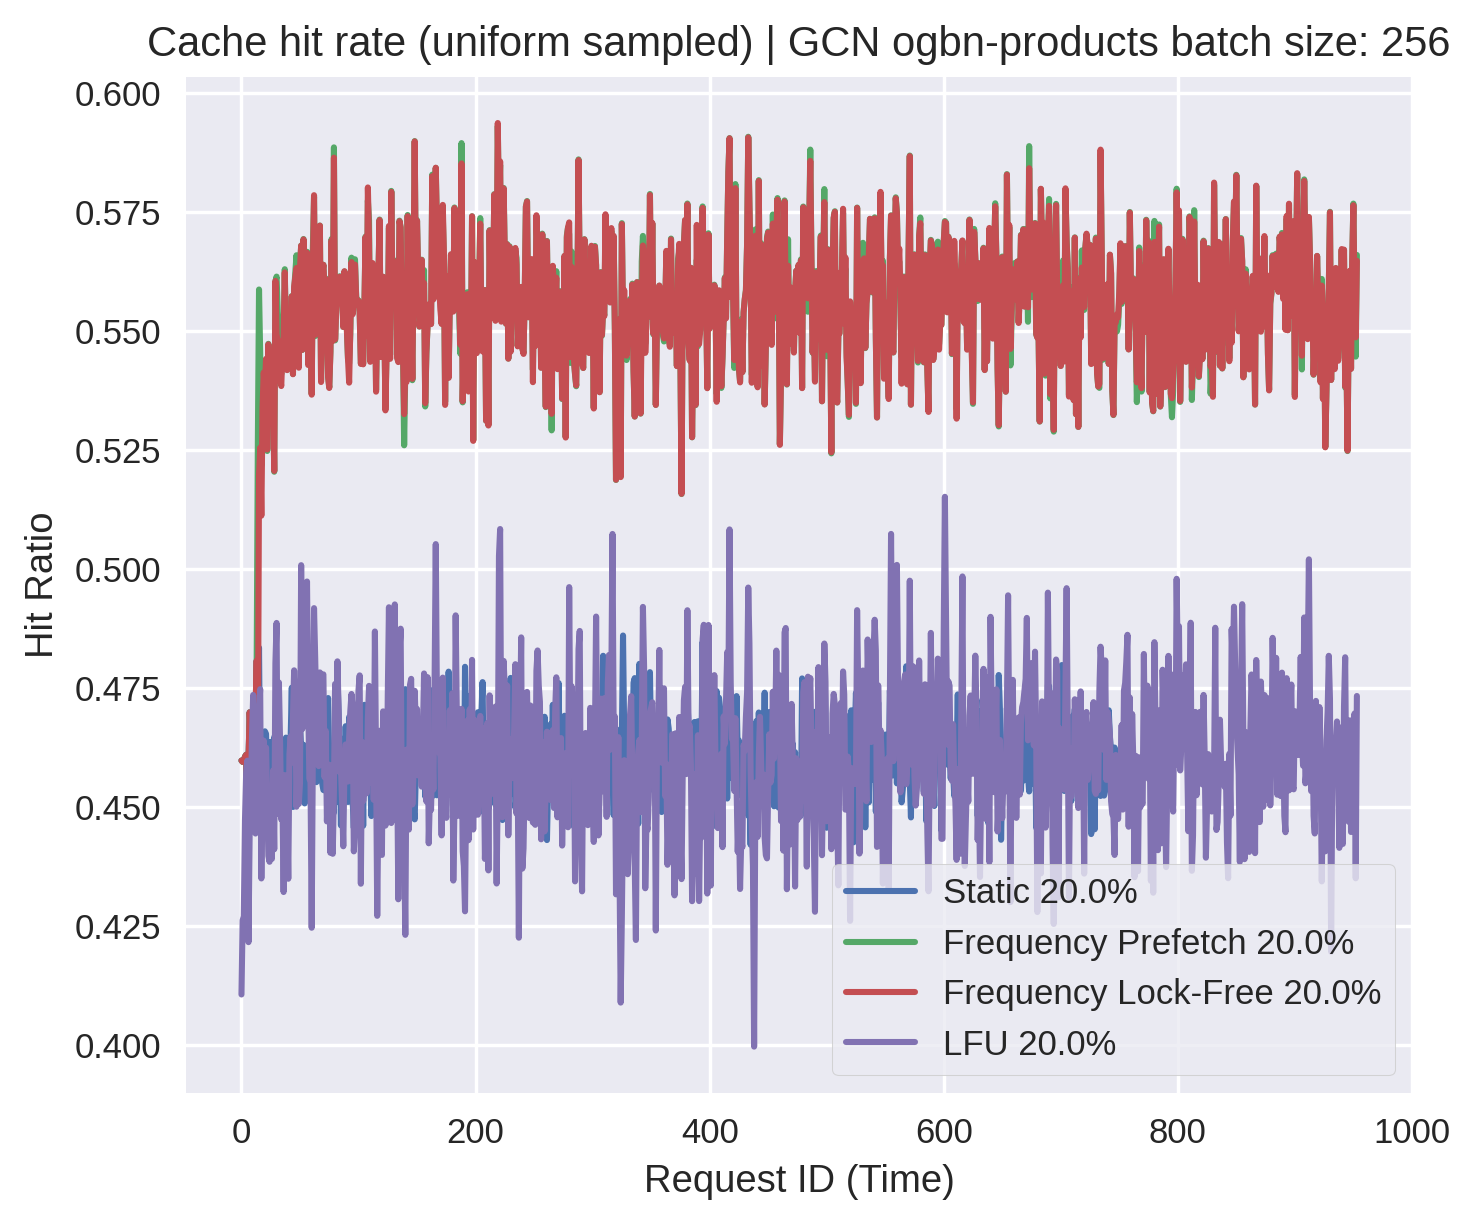
\includegraphics[width=\textwidth]{figures/CROTc0.2.png}
        \caption*{Uniformly sampled requests}
    \end{minipage}
    \hfill
    \begin{minipage}[c]{0.48\textwidth}
        \centering
        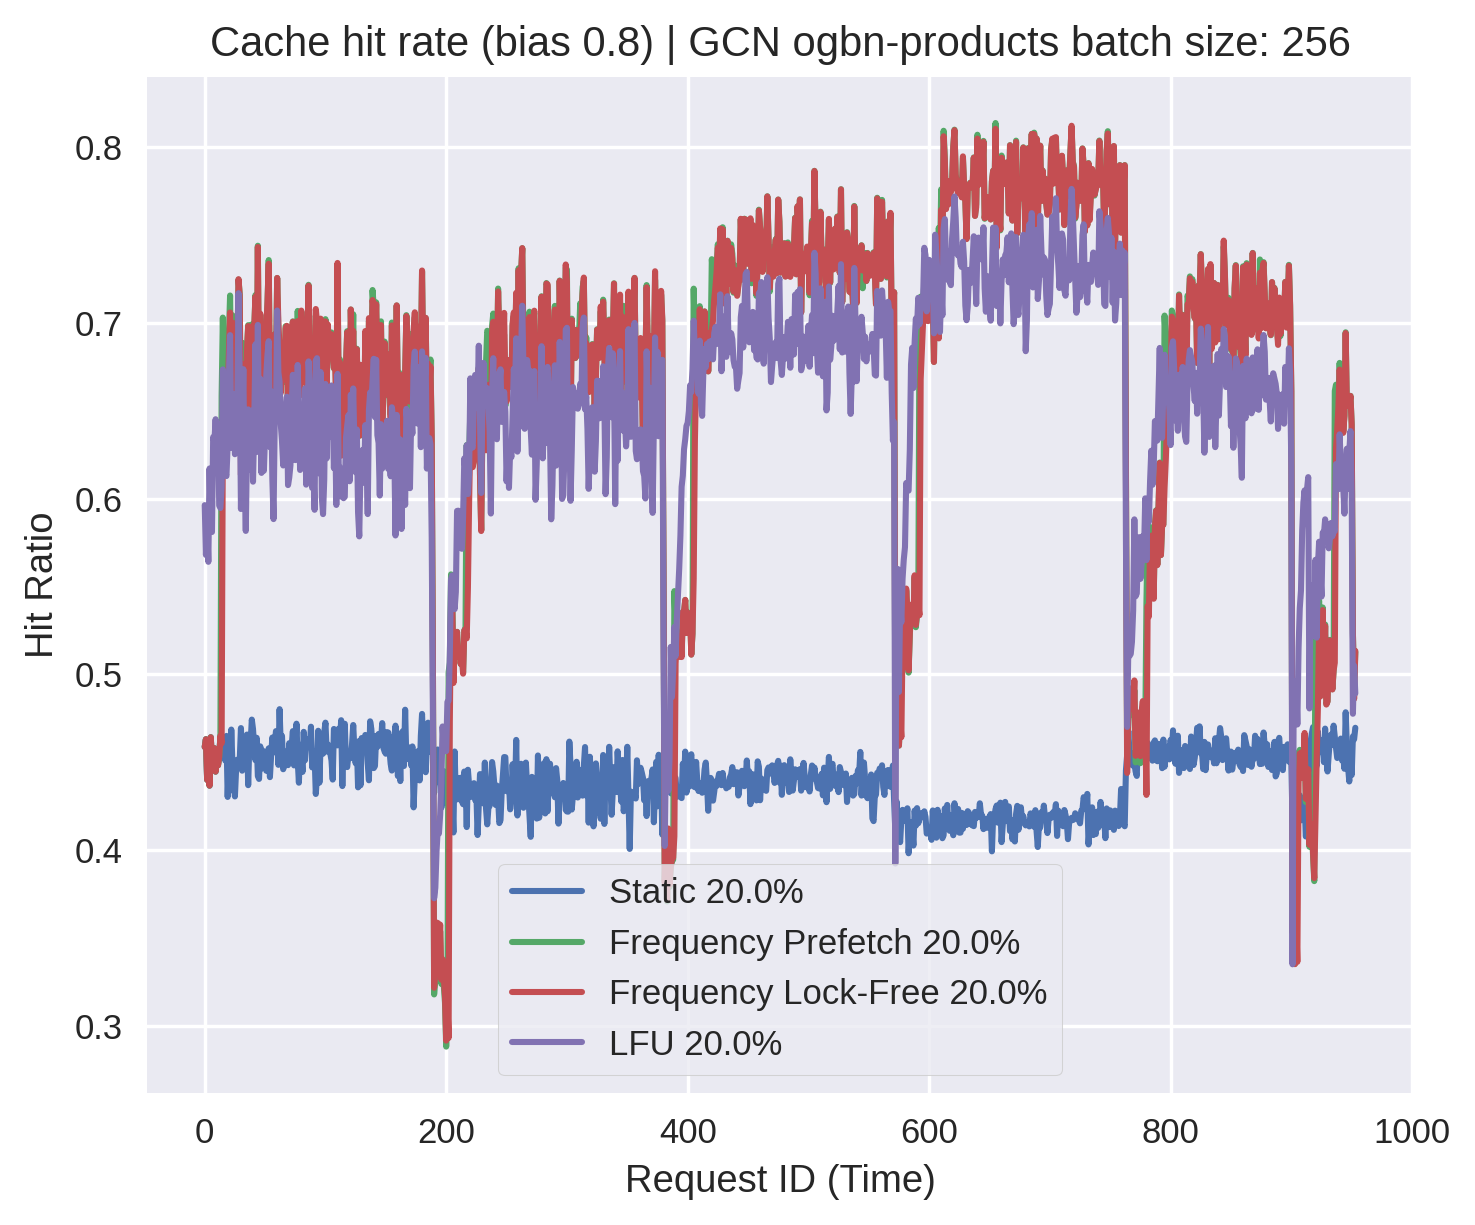
\includegraphics[width=\textwidth]{figures/CROT_biased_c0.2.png}    
        \caption*{Subgraph biased requests}
    \end{minipage}
    % 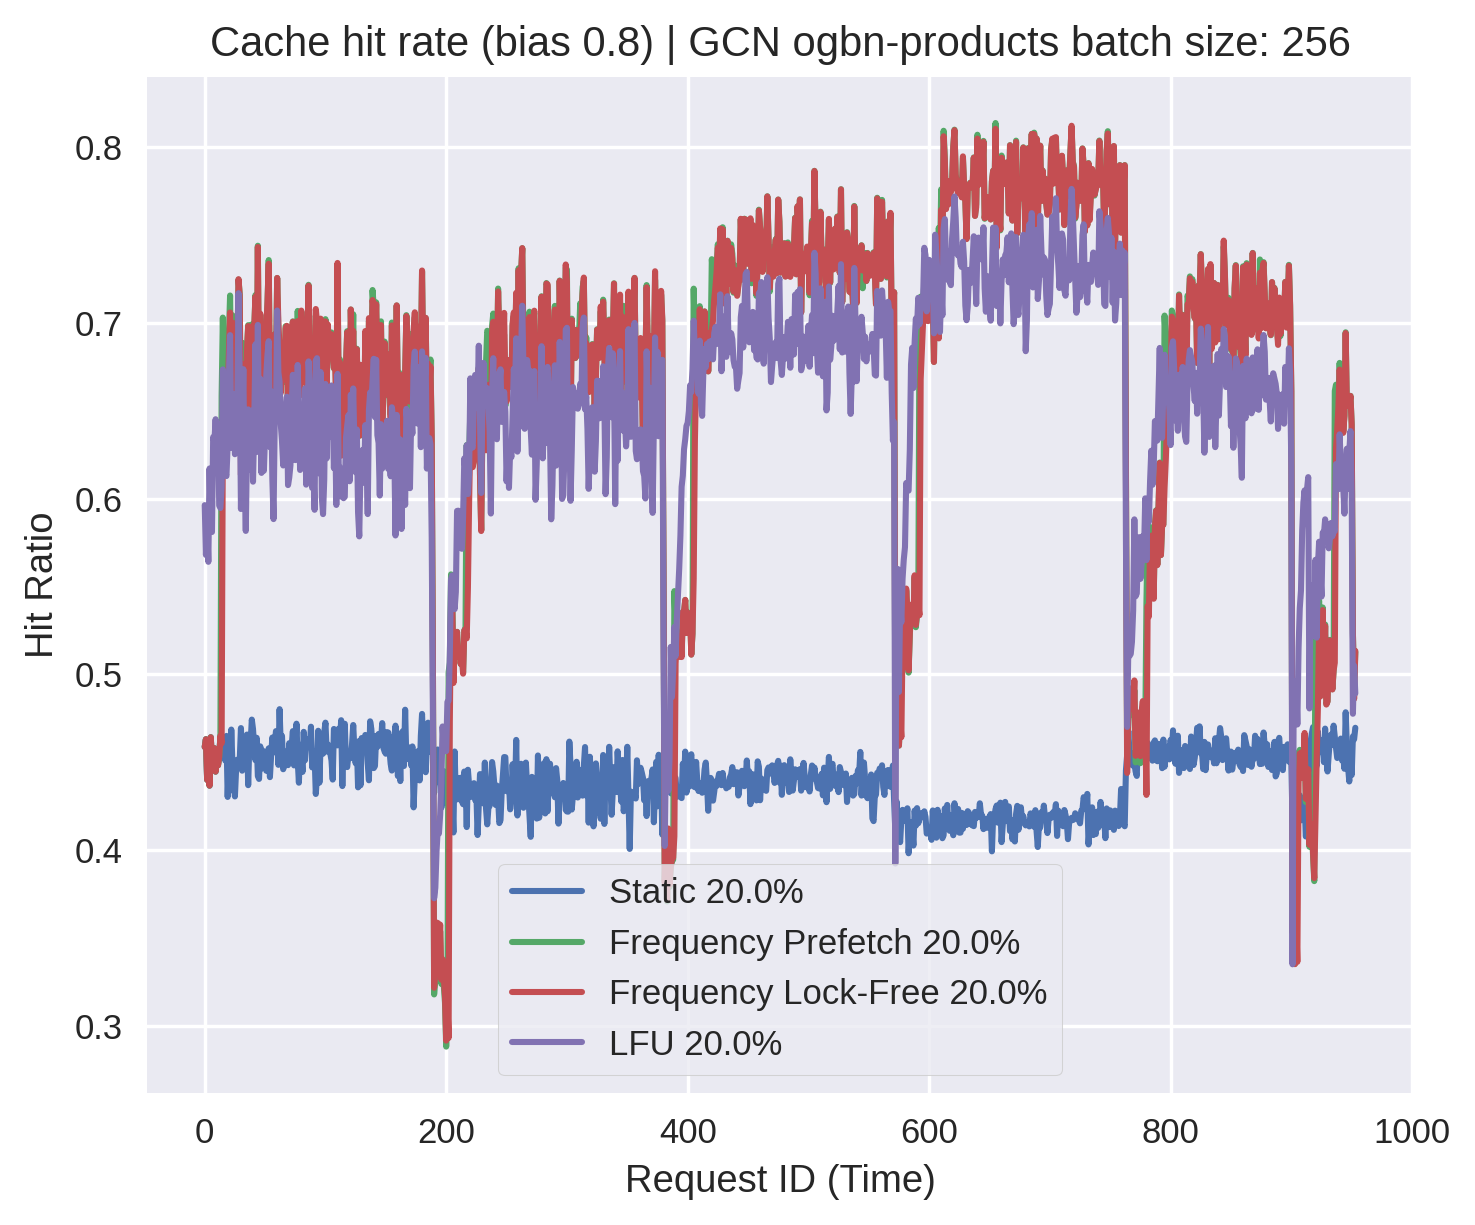
\includegraphics[width=\textwidth]{figures/CROT_biased_c0.2.png}
    \caption{Cache hit rates for ogbn-products batch size 256}
    \label{Eval: Hit Rate}
\end{figure}    

Comparing LFU and the static baseline, we immediately see that LFU struggles in the uniform sampled case since there is little cache hit rate improvement. Thus there is a median slowdown of around 10\% due to the overhead of computing LFU updates with no benefit. 

Our Frequency Prefetch strawman has the best median latencies overall, since it produces the best cache hit rates and has the same minimal overhead as a static cache. However, in the uniform sampled case the tail latency is apparent, with the 90\th percentile latency increasingly significantly due to cache updates.

The frequency-based \textit{admission} that the frequency-based policies use are crucial, as compared to LFU they offer better cache hit rates in general. While LFU can only match the static baseline cache hit rates in the uniform sampled case, by adding an admission policy enables better cache hit rates even in this difficult case. 

When examining the Frequency Lock-Free and Frequency Synchronous approaches, they both exhibit relatively little tail latency as a result of the cache candidate mechanism discussed in Section \ref{Design: Cache candidates}. In general the Frequency Synchronous approach is actually not that bad, only being 3-5\% slower on average, but Frequency Lock-Free with its asynchronous update is able to match the low-overhead median latencies of the Frequency Prefetch strawman. The time for cache updates somewhat scales with the number of nodes in the graph, and thus the disparity between asynchronous and synchronous updates will grow with scale.

%%%%%%%%%%%%%%%%%%%%%%%%%%%%%%%%%%%%%%%%%%%%%%%%%%%%%%%%%%%%%%%%%%%%%%%%
\section{Locking vs. Lock-free}
%%%%%%%%%%%%%%%%%%%%%%%%%%%%%%%%%%%%%%%%%%%%%%%%%%%%%%%%%%%%%%%%%%%%%%%%

As described in Section \ref{Design: Lock-free}, we expected that using a reader-writer lock with multiple InferenceEngines and GPUs would pose a problem for both throughput in latency. This is because cache updates would have a blocking effect on serving inference requests. To evaluate this hypothesis, we conduct several experiments comparing the Frequency Lock-free and Frequency R/W Lock policies in this section. We fix the cache size at 20\% of total graph features for all experiments.

\subsection{Throughput}
We measure the maximum possible throughput of the Static, Frequency Prefetch, Frequency Lock-free, and Frequency R/W Lock approaches.
Figure \ref{Eval: Throughput 1 GPU} shows these results using only 1 GPU and Figure \ref{Eval: Throughput 2 GPU} shows these results for 2 GPUs. In the 2 GPU case a single logical cache is partitioned between both GPUs.  

Comparing these two case, we observe that doubling the number of GPUs yields roughly linear speedup in terms of peak throughput. We do not have access to a system that has more GPUs all connected using NVLink/NVSwitch and thus do not evaluate scaling to more GPUs. Although we did have a system with four GPUs, only pairs of GPUs on different NUMA nodes were connected with NVLink. In such a situation it is better not to share a single logical cache among all GPUs, but rather have two separate caches for each pair of GPUs. Creating a logical cache between GPUs not connected using NVLink simply incurs more PCIe bus traffic.
\begin{figure}[h!]
    \centering
    \begin{minipage}[c]{0.48\textwidth}
        \centering
        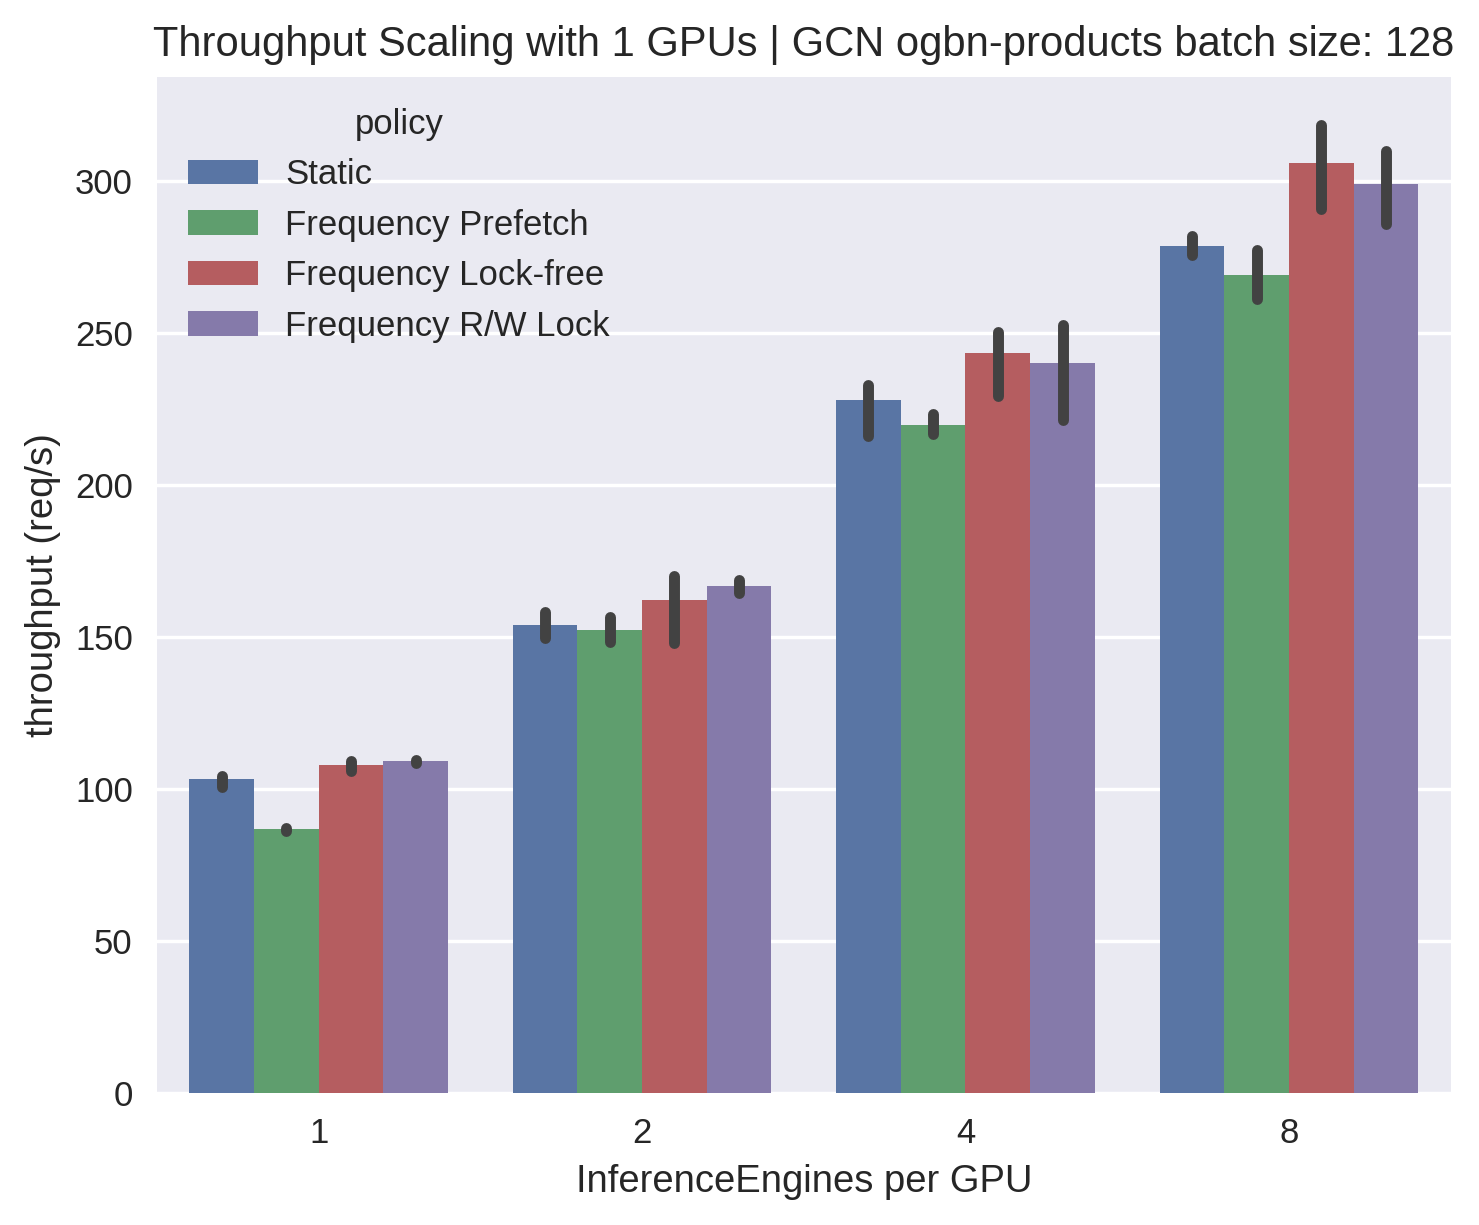
\includegraphics[width=\textwidth]{figures/throughput_GCN_uniform_pinnedc0.2_gpus_1.png}
        \caption*{Uniformly sampled requests}
    \end{minipage}
    \hfill
    \begin{minipage}[c]{0.48\textwidth}
        \centering
        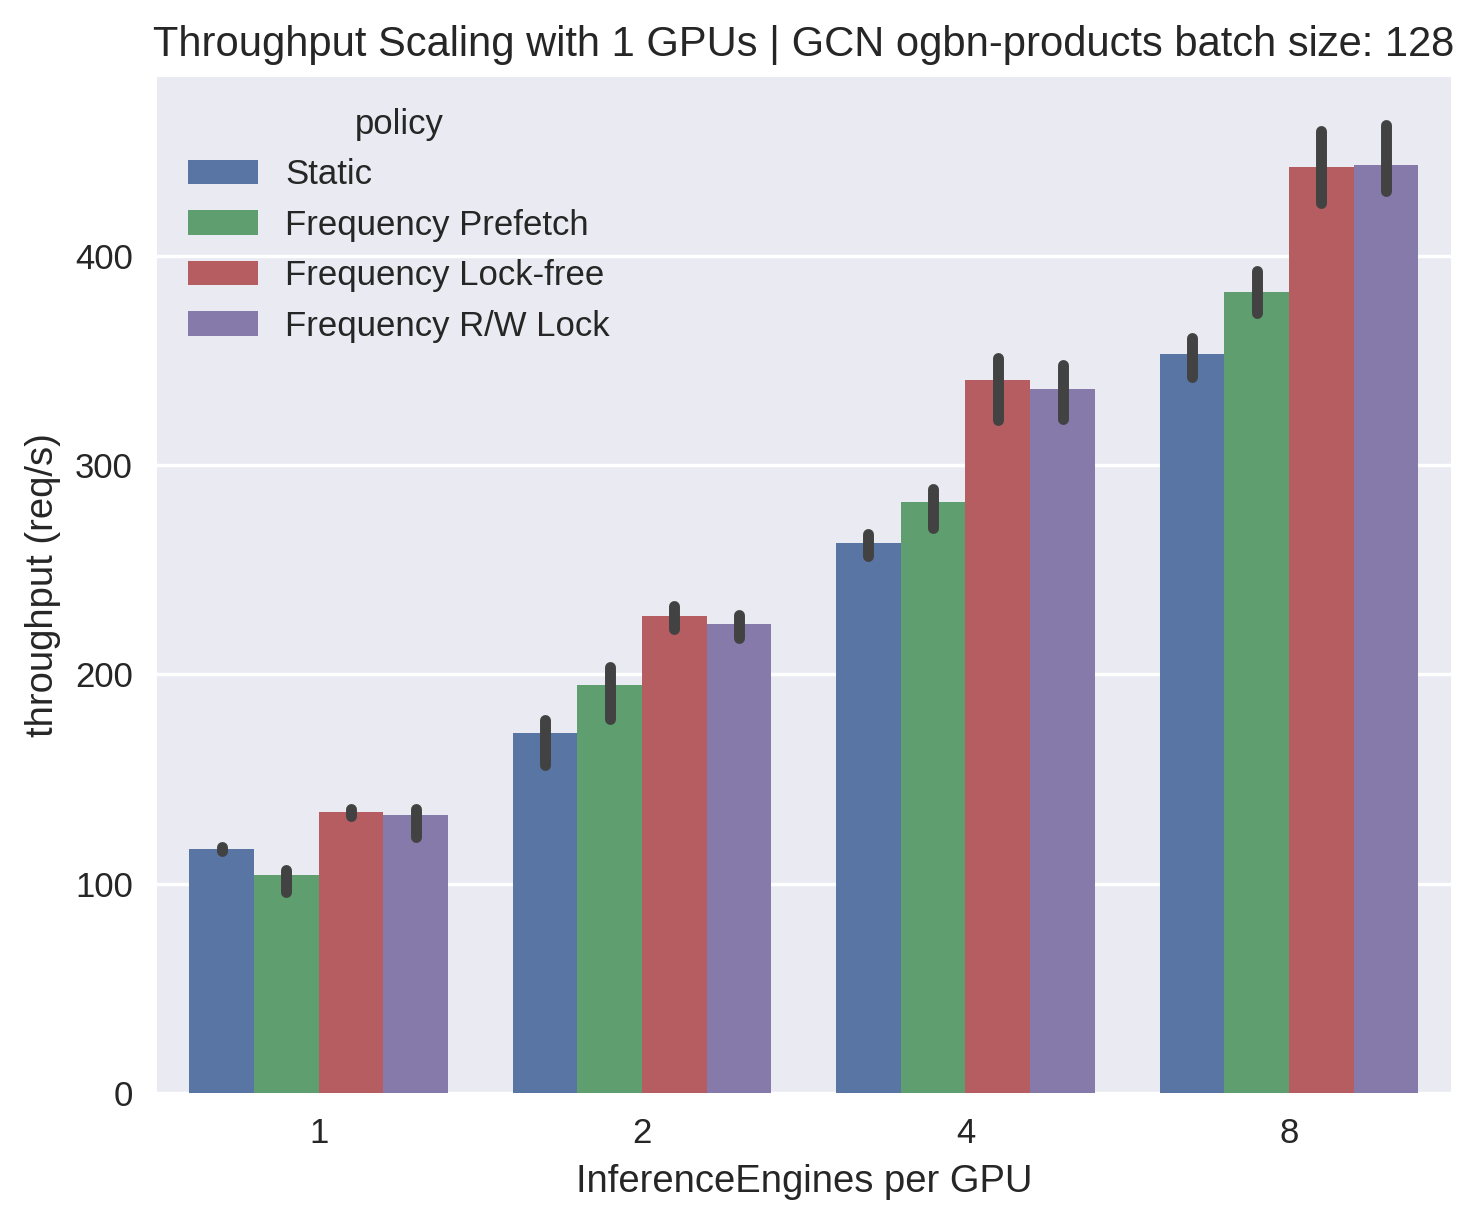
\includegraphics[width=\textwidth]{figures/throughput_GCN_bias_0.8_pinnedc0.2_gpus_1.png}    
        \caption*{Subgraph biased requests}
    \end{minipage}
    % 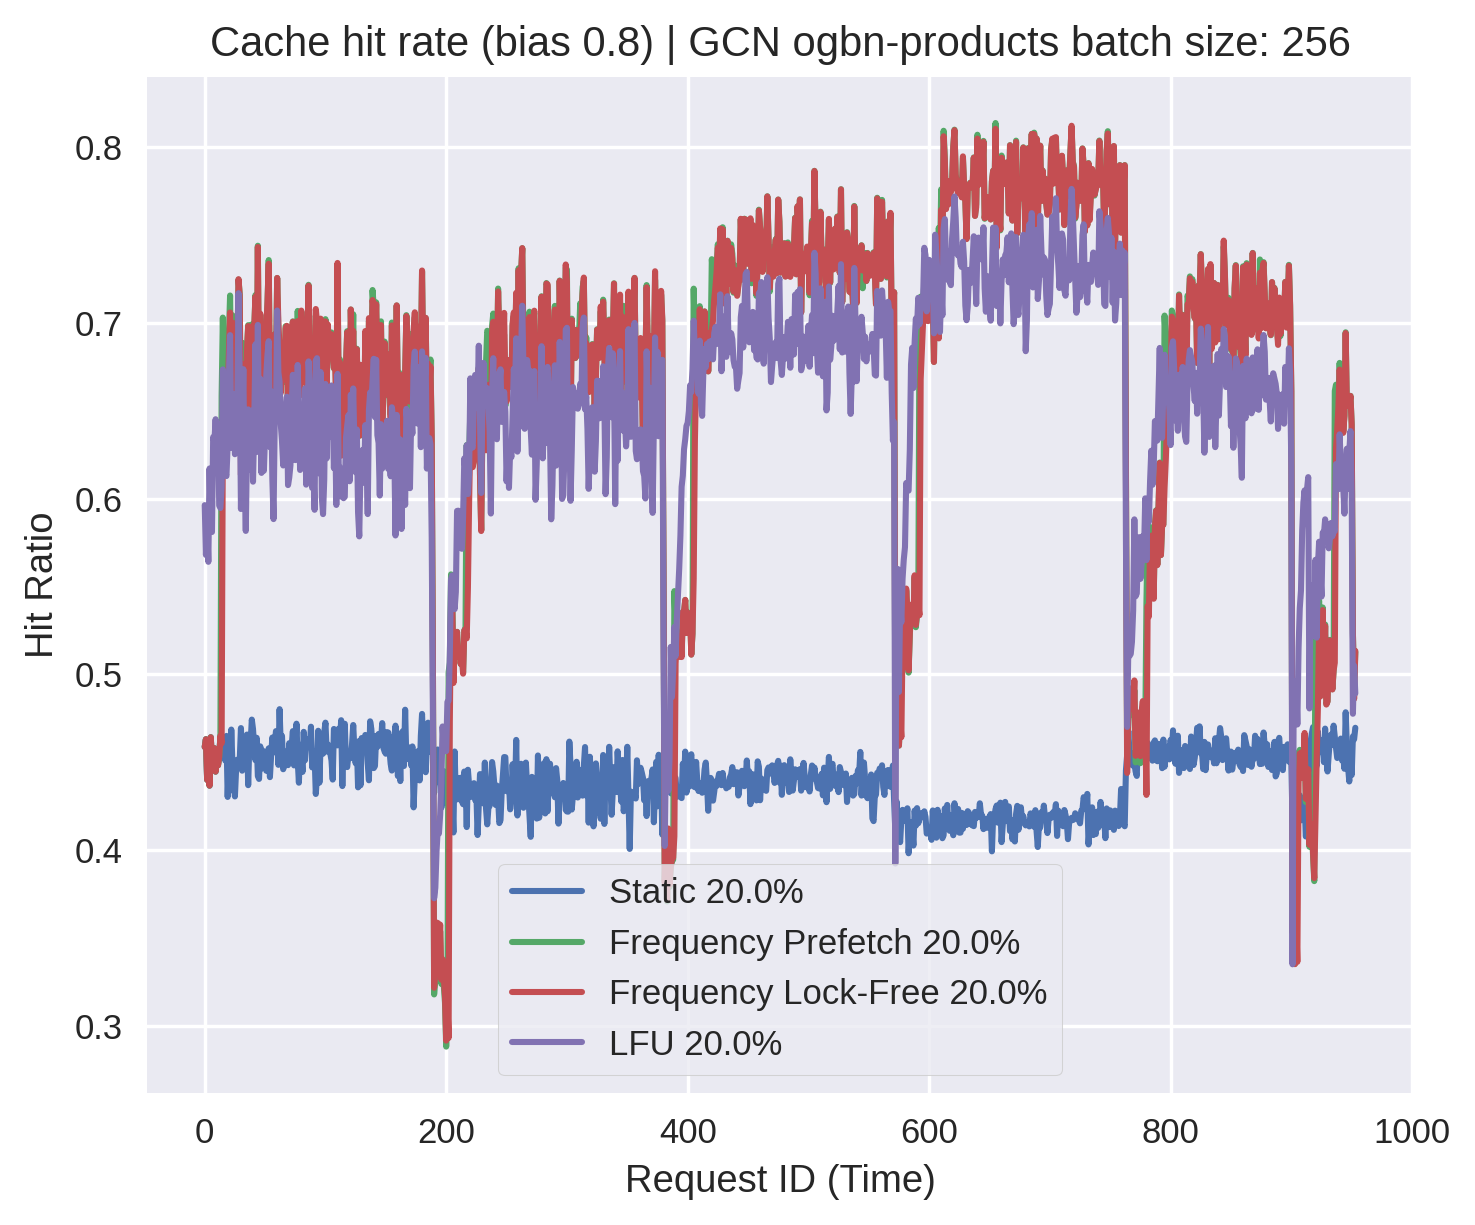
\includegraphics[width=\textwidth]{figures/CROT_biased_c0.2.png}
    \caption{Peak throughput using one GPU and varying number of InferenceEngines per GPU,}
    \label{Eval: Throughput 1 GPU}
\end{figure}    
\begin{figure}[h!]
    \centering
    \begin{minipage}[c]{0.48\textwidth}
        \centering
        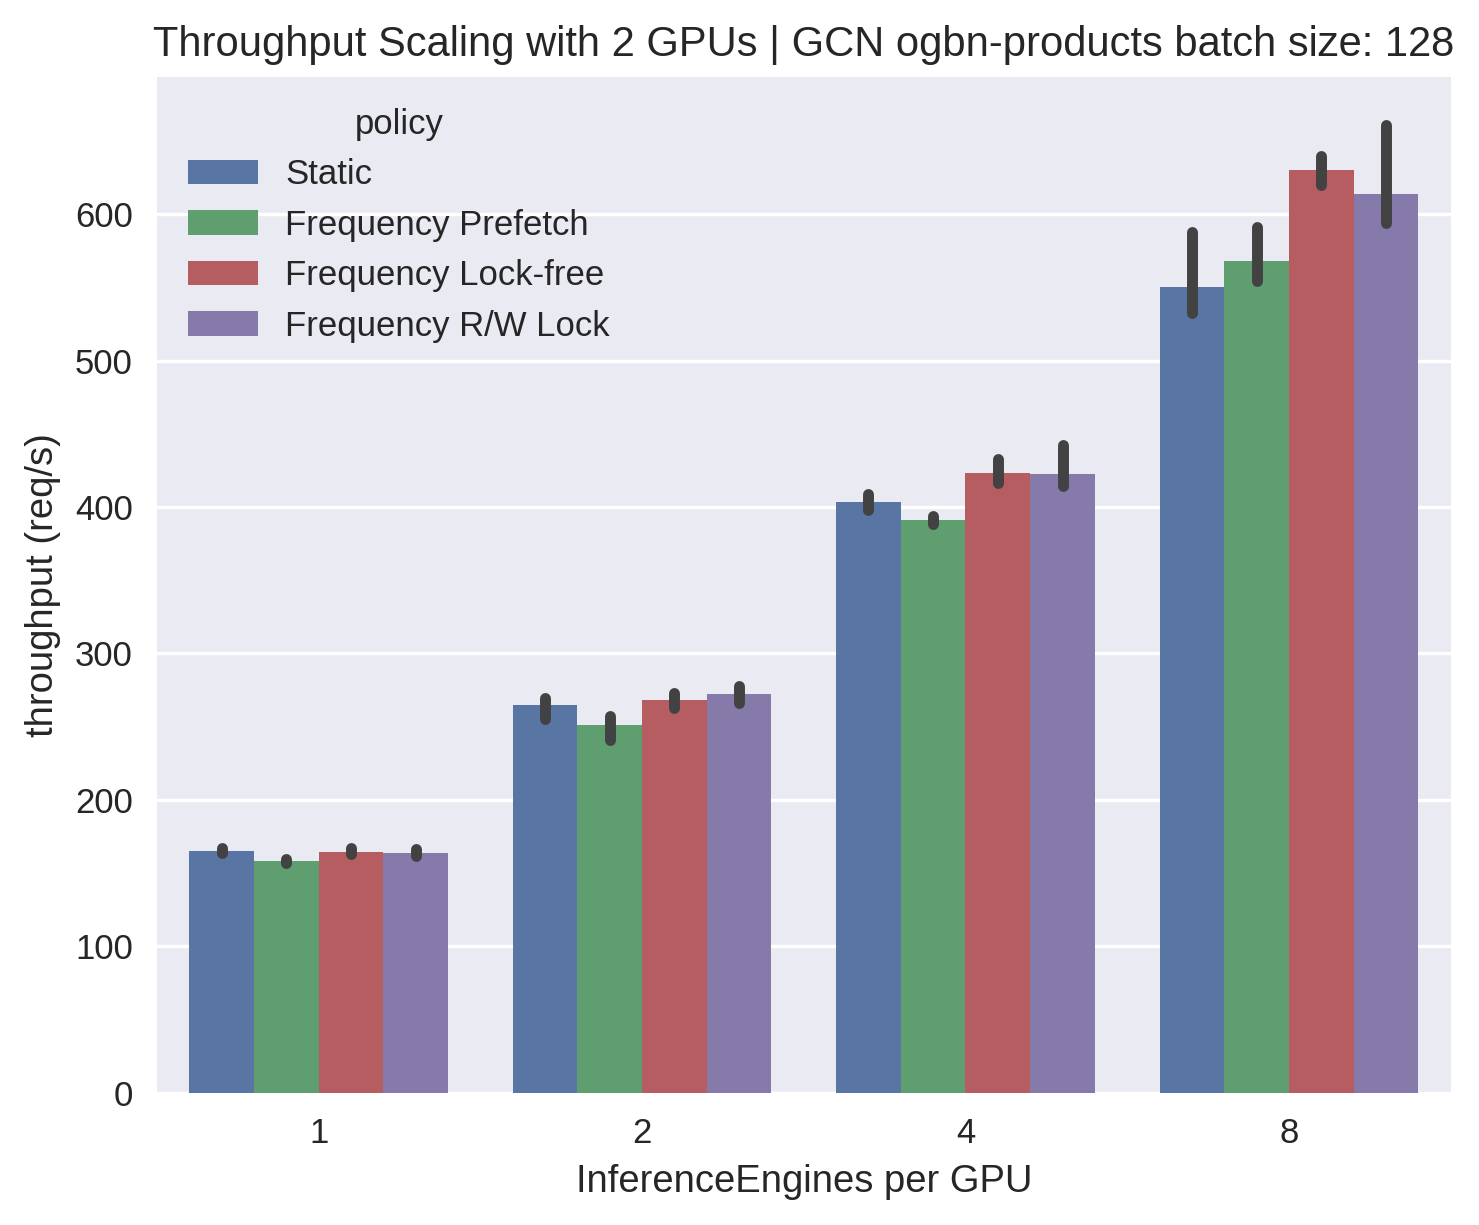
\includegraphics[width=\textwidth]{figures/throughput_GCN_uniform_pinnedc0.2_gpus_2.png}
        \caption*{Uniformly sampled requests}
    \end{minipage}
    \hfill
    \begin{minipage}[c]{0.48\textwidth}
        \centering
        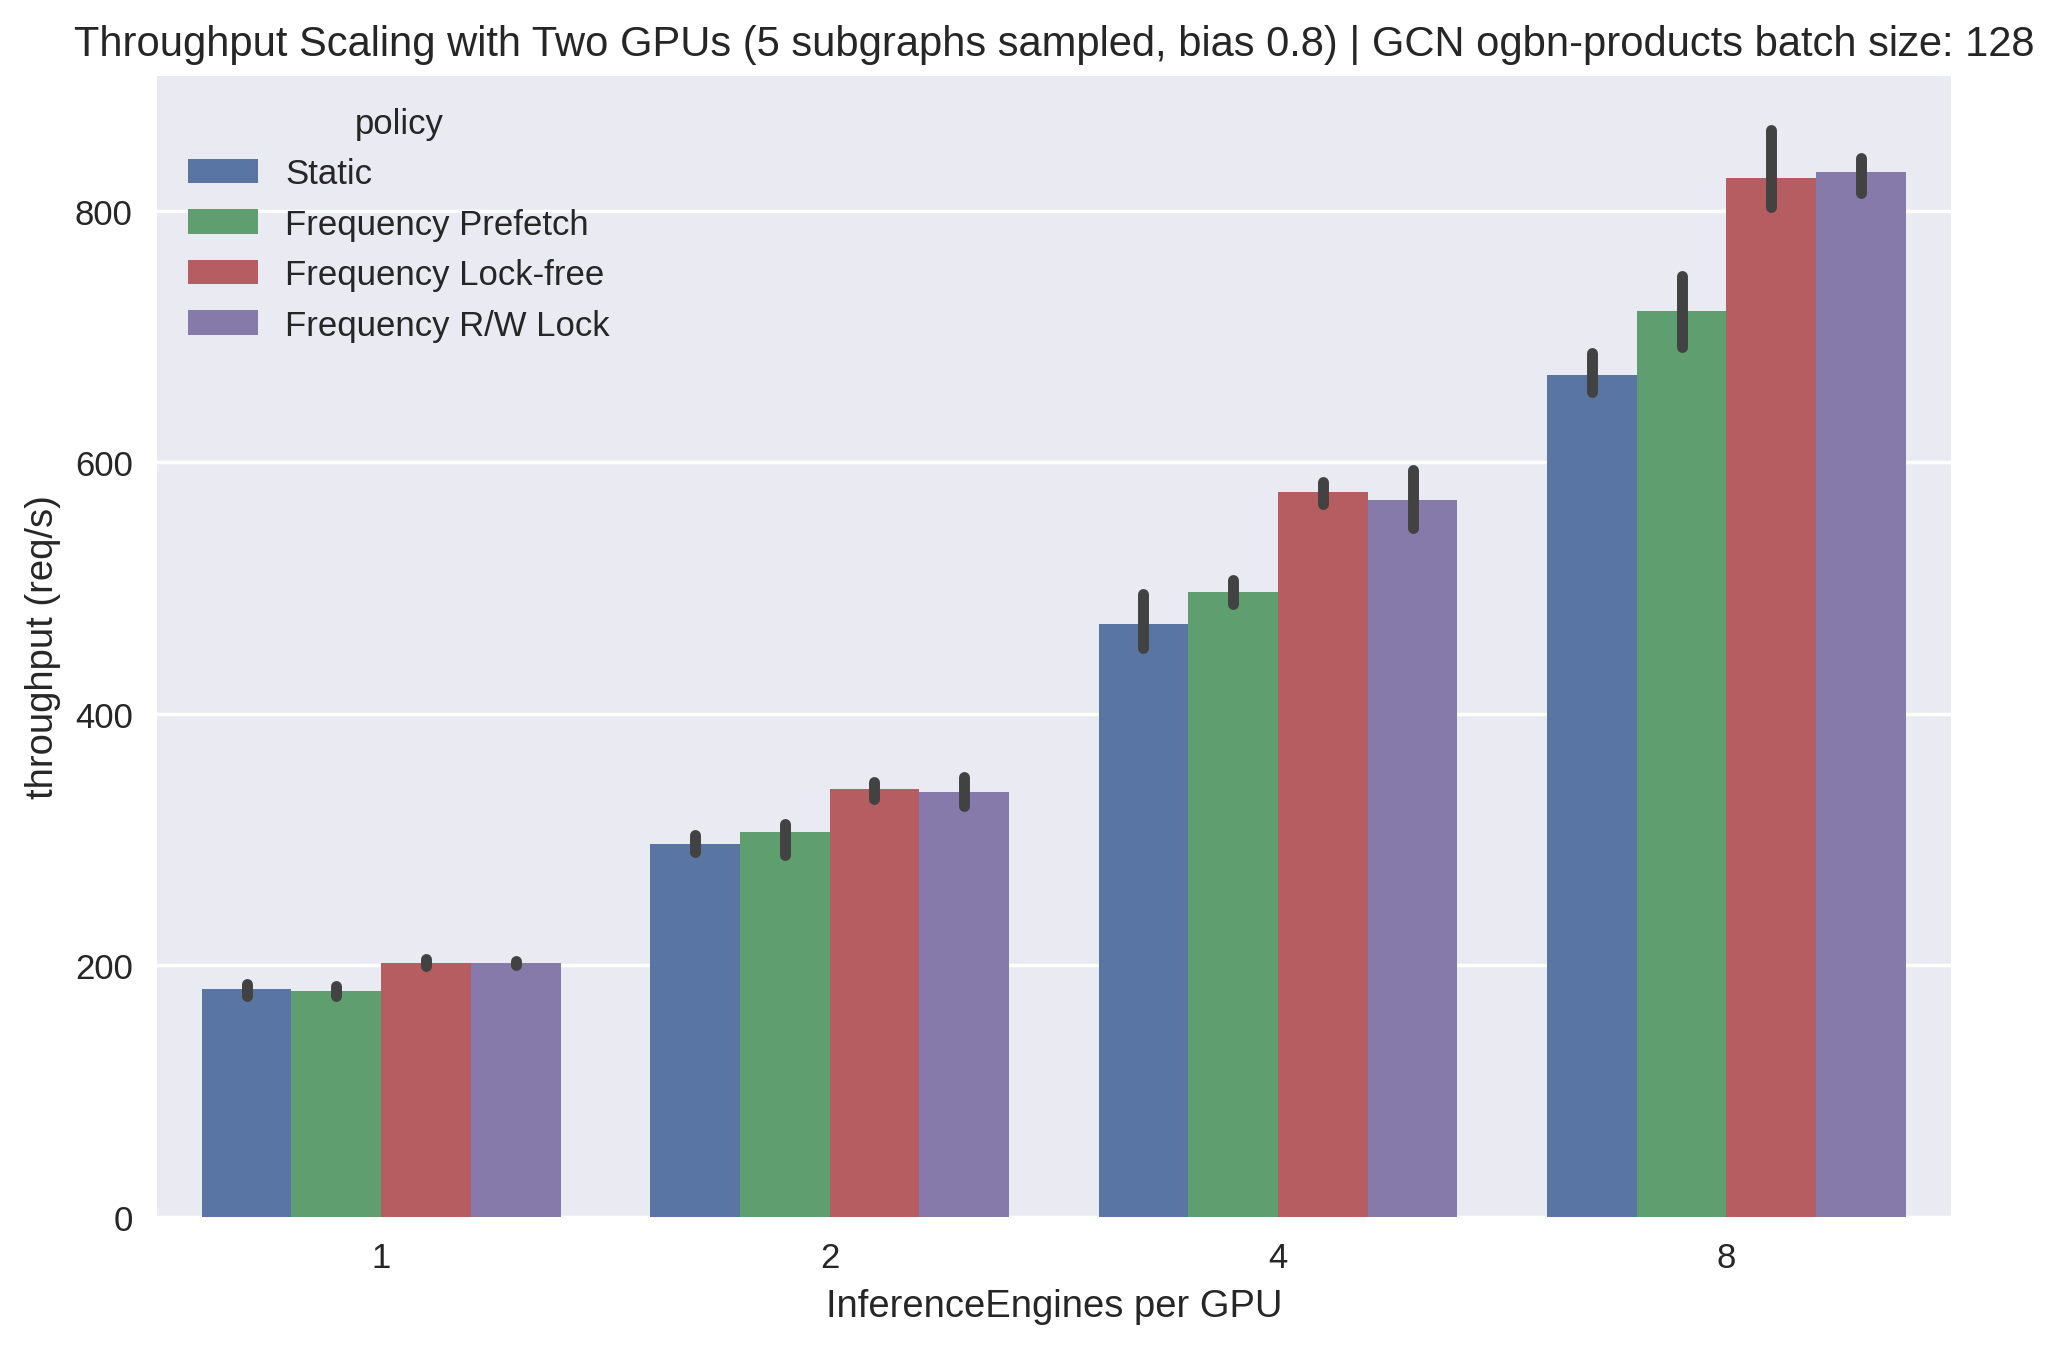
\includegraphics[width=\textwidth]{figures/throughput_GCN_bias_0.8_pinnedc0.2_gpus_2.png}    
        \caption*{Subgraph biased requests}
    \end{minipage}
    % 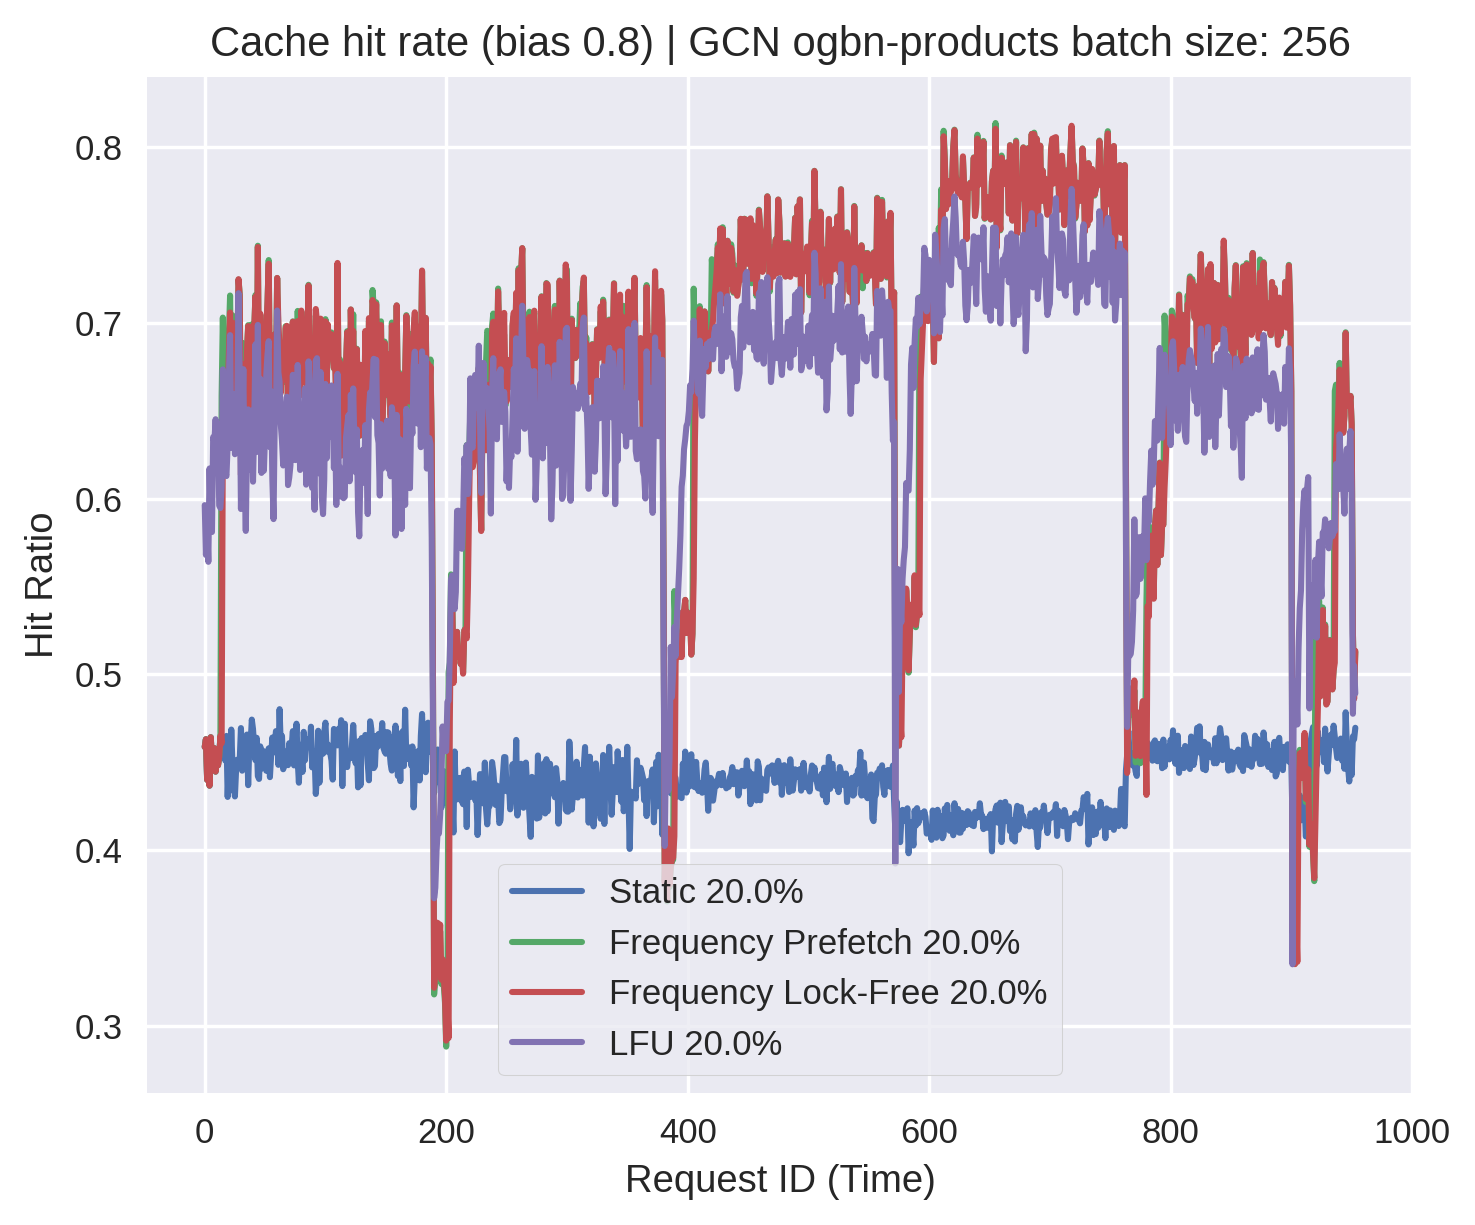
\includegraphics[width=\textwidth]{figures/CROT_biased_c0.2.png}
    \caption{Peak throughput using one GPU and varying number of InferenceEngines per GPU,}
    \label{Eval: Throughput 2 GPU}
\end{figure}   
We found that there is actually little discernable difference in peak throughput between the lock-free and R/W lock approaches, likely because of our InferenceEngine architecture. A throughput bottleneck would likely be observed if many data loaders were always trying to read from the cache, but with our architecture this only happens for a brief period of time per process. Thus there is not that much lock contention in the first place.

\subsection{P99 Latency}
Although there is little impact of lock contention on peak throughput, there is an impact on P99 latency. We conduct an experiment where we generate inference requests and vary the request rate, with delays between requests drawn from an exponential distribution. Figure \ref{Eval: P99 latency} shows P99 latencies for various policies when the request rate varies. In this test we use both GPUs and eight InferenceEngines per GPU. Note the log scale.

\begin{figure}[h!]
    \centering
    \begin{minipage}[c]{0.48\textwidth}
        \centering
        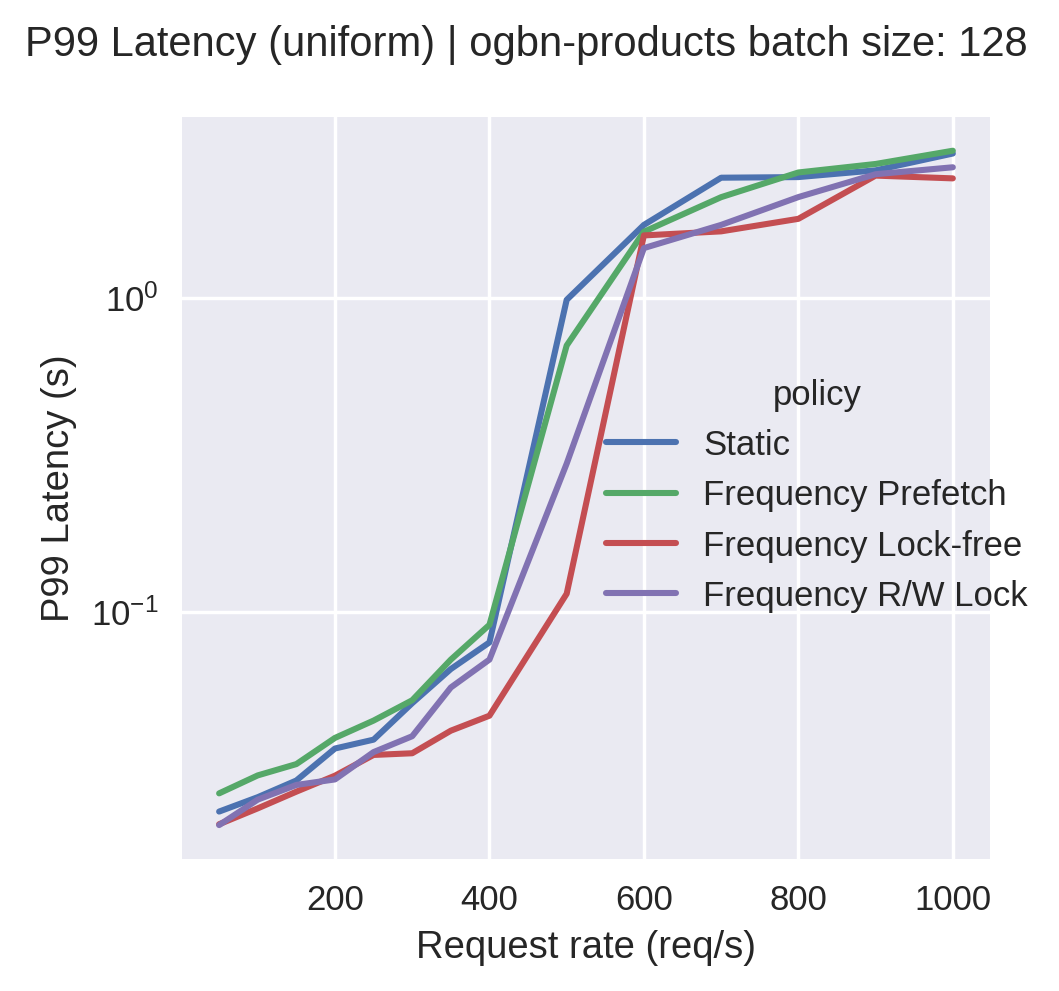
\includegraphics[width=\textwidth]{figures/P99_latency_GCN_uniform_pinnedc0.2_gpus_3.png}
        \caption*{Uniformly sampled requests}
    \end{minipage}
    \hfill
    \begin{minipage}[c]{0.48\textwidth}
        \centering
        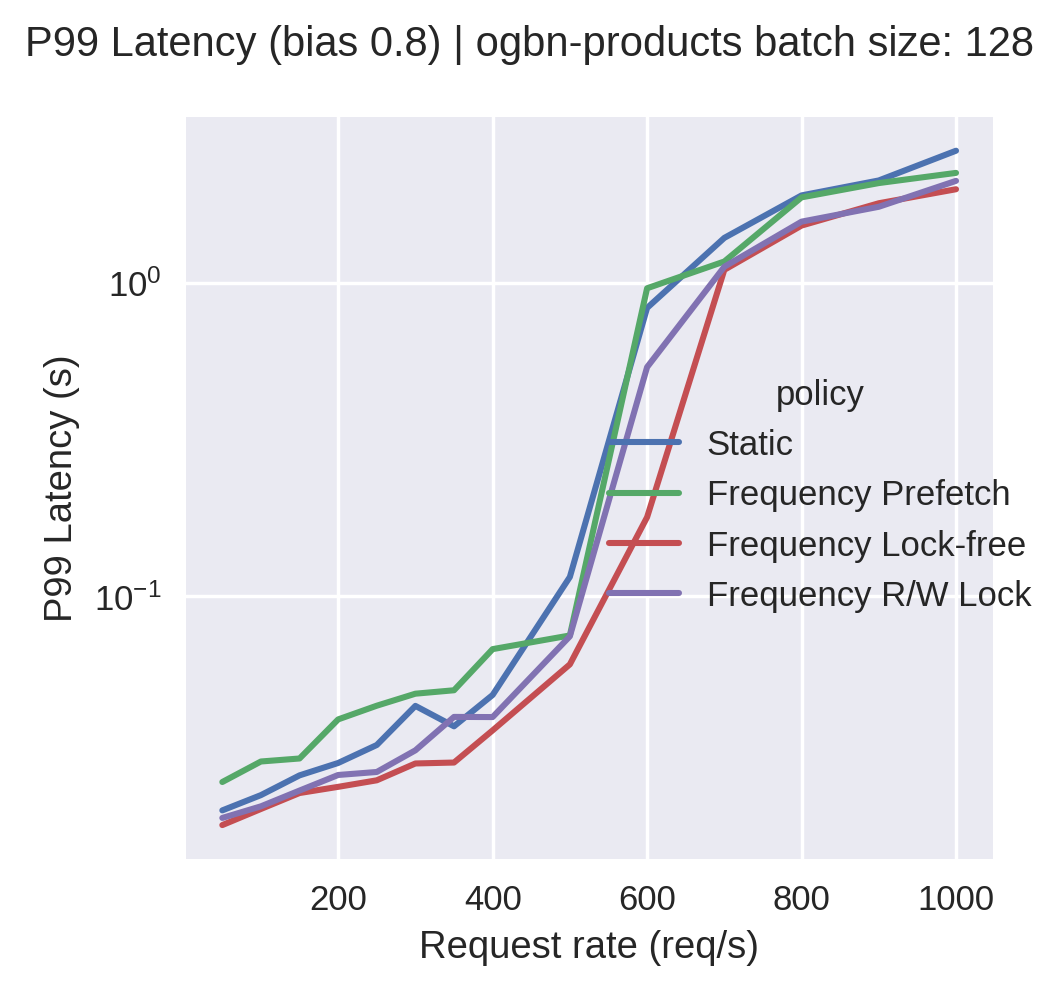
\includegraphics[width=\textwidth]{figures/P99_latency_GCN_bias_0.8_pinnedc0.2_gpus_3.png}    
        \caption*{Subgraph biased requests}
    \end{minipage}
    \caption{99\th percentile latencies for varying request rates. Tested on system using both GPUs and eight InferenceEngines per GPU.}
    \label{Eval: P99 latency}
\end{figure}  
We see that using the lock-free approach reduces P99 latency across the board. Lock contention can occasionally produce slow responses, which the lock-free approach avoids.

\subsection{Lock Conflict Microbenchmark} \label{Eval: microbenchmark}
We also conduct a small microbenchmark to identify the scale potential lock contention in a fully pipelined system. 
We remove the sampling and model execution stages from the InferenceEngines and instead send requests that already contain $k$-hop neighborhoods at maximum throughput.
We then measure the amount of time spent waiting to acquire read locks for the Frequency R/W lock policy. 
In this experiment we use a machine that is equivalent in all ways to our original machine but has two additional GPUs. Figure \ref{Eval: Lock conflict microbenchmark} illustrates these results. Note the log scale.
\begin{figure}[h!]
    \centering
    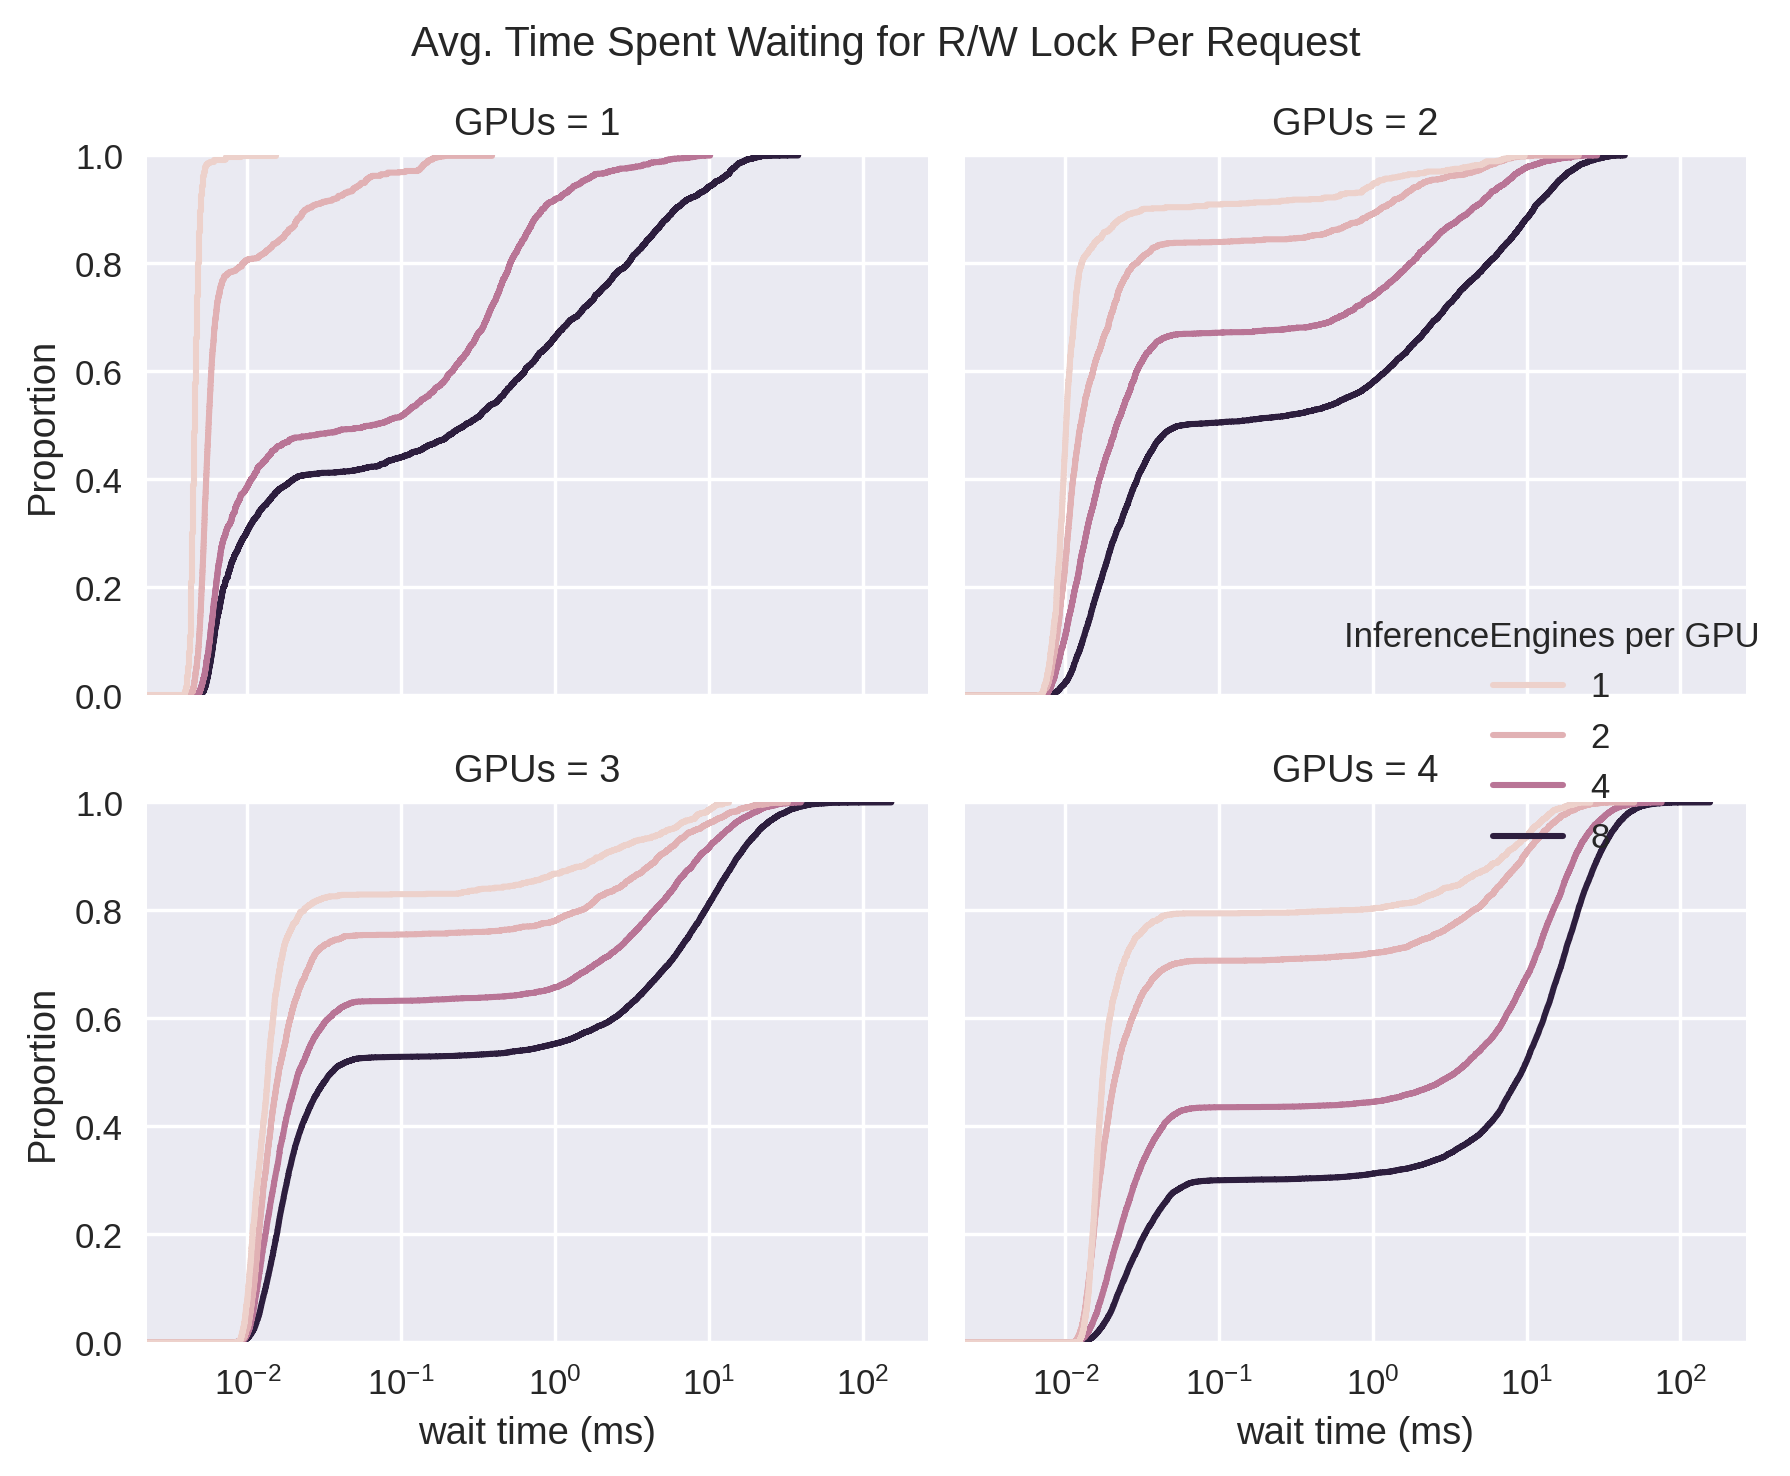
\includegraphics[width=0.8\textwidth]{figures/Lock_Conflicts.png}
    
    \caption{Lock contention microbenchmark.}
    \label{Eval: Lock conflict microbenchmark}
\end{figure}    
By increasing the number of GPUs, the number of cache writers (updaters) at a given time increases. Thus, the likelihood of a cache read being blocked by a cache update increases. Naturally, this is also proportional to the number of data loaders (InferenceEngines) present in the system. 

This result points to our masked cache approach becoming more important in large-scale system with many GPUs.

